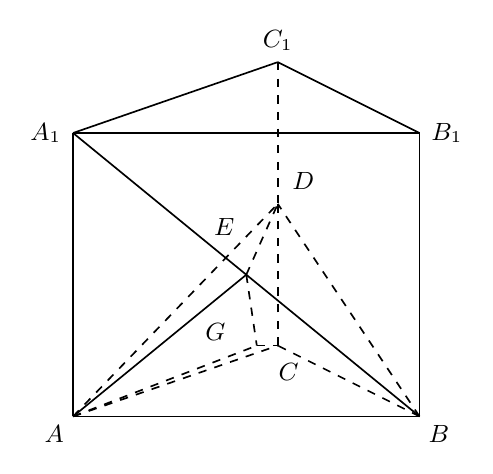
\begin{tikzpicture}[scale=1,line width=.6pt]
\tikzset{lbl/.style={font=\small,inner sep=1pt}}
\coordinate (A) at (0,0);
\coordinate (B) at (4.4,0);
\coordinate (C) at (2.6,0.9);
\coordinate (A1) at (0,3.6);
\coordinate (B1) at (4.4000000000,3.6000000000);
\coordinate (C1) at (2.6000000000,4.5000000000);
\coordinate (D) at (2.6000000000,2.7000000000);
\coordinate (E) at (2.2000000000,1.8000000000);
\coordinate (G) at (2.3333333333,0.9000000000);
% solid outline + top
\draw (A)--(B);
\draw (B)--(B1);
\draw (B1)--(A1);
\draw (A1)--(A);
\draw (A1)--(C1);
\draw (B1)--(C1);
\draw (A1)--(B);
\draw (A)--(E);
% dashed hidden
\draw[dashed] (A)--(C);
\draw[dashed] (B)--(C);
\draw[dashed] (C)--(D);
\draw[dashed] (C1)--(D);
\draw[dashed] (A)--(D);
\draw[dashed] (B)--(D);
\draw[dashed] (E)--(D);
\draw[dashed] (E)--(G);
\draw[dashed] (A)--(G);
\draw[dashed] (G)--(C);
\node[lbl,below left=2pt] at (A) {$A$};
\node[lbl,below right=2pt] at (B) {$B$};
\node[lbl,below right=2pt,xshift=-3pt,yshift=-3pt] at (C) {$C$};
\node[lbl,left=3pt] at (A1) {$A_{1}$};
\node[lbl,right=3pt] at (B1) {$B_{1}$};
\node[lbl,above=3pt] at (C1) {$C_{1}$};
\node[lbl,above right=4pt] at (D) {$D$};
\node[lbl,above left=5pt,xshift=2pt,yshift=8pt] at (E) {$E$};
\node[lbl,left=5pt,xshift=-5pt,yshift=5pt] at (G) {$G$};
\end{tikzpicture}